\documentclass[12pt,a4paper]{article}

\usepackage[utf8]{inputenc}
\usepackage{polski}
\usepackage[polish]{babel}

\usepackage[left=2.5cm, right=2.5cm, top=2.5cm, bottom=2.5cm]{geometry}
\usepackage{indentfirst}

\usepackage{graphicx}

\begin{document}
	
		\begin{titlepage}

		\vspace*{1cm}

	    \begin{center}
		    \small
		    Politechnika Wrocławska\\
		    Wydział Elektroniki\\
		    Podstawy Technik Mikroprocesorowych
	    \end{center}

	    \vspace{3cm}

		\noindent\rule{\linewidth}{0.4mm}
	    \begin{center}
			\LARGE \textsc{Mikroprocesorowy Sterownik Śledzący Anteny Satelitarne} !!!!
	    \end{center}
		\noindent\rule{\linewidth}{0.4mm}

		\vspace{0.5cm}

%Do poprawienia na pierwszej stronie.
%http://en.wikibooks.org/wiki/LaTeX/Title_Creation
	    \begin{flushright}
			\begin{minipage}{6cm}
				\textit{\small Autor:}\\
				\normalsize \textsc{Paweł Szwagierek}
			\end{minipage}
			\vspace{3cm}
			{\small Prowadzący:}\\
			dr inż. Jerzy Greblicki
	    \end{flushright}

	    \vspace*{\stretch{6}}

	    \begin{center}
		    \today
	    \end{center}	
    \end{titlepage}


	\tableofcontents
	\clearpage

	\section{Wstęp}
	Celem projektu jest zbudowanie sterownika rotora antenowego dla zastosowań krótkofalarskich. Sterownik mikroprocesorowy powinien umieć skierować antenę w ustalonym kierunku według podanych współrzędnych horyzontalnych (Azymut i Elewacja).

	\section{Protokół DDE}

	\section{Przygotowanie oprogramowania po stronie komputera}
		
		\subsection{Konfiguracja programu Orbitron}
		Koniecznymi ustawieniami w programie Orbitron są:
		\begin{itemize}
			\item Współrzędne geograficzne położenia anteny
			\item Wysokość nad poziomem morza (konieczna do korekcji elewacji)
			\item Wybór sterownika DDE
		\end{itemize}
		Współrzędne geograficzne oraz wysokość ustawia się w zakładce Lokalizacja przedstawionej na rysunku~\ref{fig:location_settings}. Długość i szerokość geograficzną można wpisać ręcznie w pola tekstowe lub wybrać z już zdefiniowanych profili. Wysokość nad poziomem morza należy wpisać ręcznie w pole tekstowe. W
		\begin{figure}[!htb]
			\begin{center}
				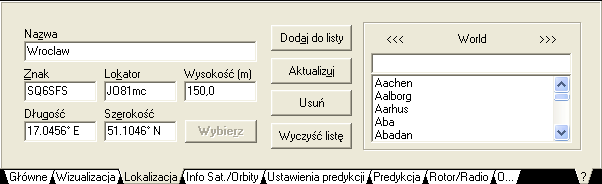
\includegraphics[scale=0.7]{screen1}
			\end{center}
			\caption{Orbitron - ustawienia lokalizacji}
			\label{fig:location_settings}
		\end{figure}

		\subsection{Powiązanie programu Orbitron ze sterownikiem WispDDE}
		\subsection{Konfiguracja sterownika WispDDE}

	Dokumentacja przygotowana w \LaTeXe
		
	
		\subsection{Programowanie mikrokontrolera STM32F0 - Discovery}
		\begin{itemize}
			\item ST-Link driver - zainstaluj sterownik -> menadżer urządzeń ST-Link USB - aktualizuj -> zainstaluj mimo to.
		\end{itemize}

	

	\section{Opracowanie projektu}

		\subsection{Przygotowanie projektu w programie Keil}
		Pierwszym ważnym krokiem jest stworzenie kompilującego się pustego projektu zawierającego wszystkie potrzebne biblioteki. Po uruchomieniu programu zobaczymy puste okna.
	
	\section{Wnioski oraz podsumowanie}
	***WWW***

\end{document} %End of document.